\documentclass{article}


%--------------------------------------------------------------------------
%--------------------------------------------------------------------------
%----------------------- INCLUDES -----------------------------------------
%--------------------------------------------------------------------------
%--------------------------------------------------------------------------

%%%%%%%%%%%%%%%%%%%%%%%%%%%%%%%%%%%%%%%%%
% Lachaise Assignment
% Structure Specification File
% Version 1.0 (26/6/2018)
%
% This template originates from:
% http://www.LaTeXTemplates.com
%
% Authors:
% Marion Lachaise & François Févotte
% Vel (vel@LaTeXTemplates.com)
%
% License:
% CC BY-NC-SA 3.0 (http://creativecommons.org/licenses/by-nc-sa/3.0/)
% 
%%%%%%%%%%%%%%%%%%%%%%%%%%%%%%%%%%%%%%%%%

%----------------------------------------------------------------------------------------
%	PACKAGES AND OTHER DOCUMENT CONFIGURATIONS
%----------------------------------------------------------------------------------------

\usepackage{amsmath,amsfonts,stmaryrd,amssymb} % Math packages

\usepackage{enumerate} % Custom item numbers for enumerations

\usepackage[ruled]{algorithm2e} % Algorithms

\usepackage[framemethod=tikz]{mdframed} % Allows defining custom boxed/framed environments

\usepackage{listings} % File listings, with syntax highlighting
\lstset{
	basicstyle=\ttfamily, % Typeset listings in monospace font
}

%----------------------------------------------------------------------------------------
%	DOCUMENT MARGINS
%----------------------------------------------------------------------------------------

\usepackage{geometry} % Required for adjusting page dimensions and margins

\geometry{
	paper=a4paper, % Paper size, change to letterpaper for US letter size
	top=2.5cm, % Top margin
	bottom=3cm, % Bottom margin
	left=2.5cm, % Left margin
	right=2.5cm, % Right margin
	headheight=14pt, % Header height
	footskip=1.5cm, % Space from the bottom margin to the baseline of the footer
	headsep=1.2cm, % Space from the top margin to the baseline of the header
	%showframe, % Uncomment to show how the type block is set on the page
}

%----------------------------------------------------------------------------------------
%	FONTS
%----------------------------------------------------------------------------------------

\usepackage[utf8]{inputenc} % Required for inputting international characters
\usepackage[T1]{fontenc} % Output font encoding for international characters

\usepackage{XCharter} % Use the XCharter fonts

%----------------------------------------------------------------------------------------
%	COMMAND LINE ENVIRONMENT
%----------------------------------------------------------------------------------------

% Usage:
% \begin{commandline}
%	\begin{verbatim}
%		$ ls
%		
%		Applications	Desktop	...
%	\end{verbatim}
% \end{commandline}

\mdfdefinestyle{commandline}{
	leftmargin=10pt,
	rightmargin=10pt,
	innerleftmargin=15pt,
	middlelinecolor=black!50!white,
	middlelinewidth=2pt,
	frametitlerule=false,
	backgroundcolor=black!5!white,
	frametitle={Command Line},
	frametitlefont={\normalfont\sffamily\color{white}\hspace{-1em}},
	frametitlebackgroundcolor=black!50!white,
	nobreak,
}

% Define a custom environment for command-line snapshots
\newenvironment{commandline}{
	\medskip
	\begin{mdframed}[style=commandline]
}{
	\end{mdframed}
	\medskip
}

%----------------------------------------------------------------------------------------
%	FILE CONTENTS ENVIRONMENT
%----------------------------------------------------------------------------------------

% Usage:
% \begin{file}[optional filename, defaults to "File"]
%	File contents, for example, with a listings environment
% \end{file}

\mdfdefinestyle{file}{
	innertopmargin=1.6\baselineskip,
	innerbottommargin=0.8\baselineskip,
	topline=false, bottomline=false,
	leftline=false, rightline=false,
	leftmargin=2cm,
	rightmargin=2cm,
	singleextra={%
		\draw[fill=black!10!white](P)++(0,-1.2em)rectangle(P-|O);
		\node[anchor=north west]
		at(P-|O){\ttfamily\mdfilename};
		%
		\def\l{3em}
		\draw(O-|P)++(-\l,0)--++(\l,\l)--(P)--(P-|O)--(O)--cycle;
		\draw(O-|P)++(-\l,0)--++(0,\l)--++(\l,0);
	},
	nobreak,
}

% Define a custom environment for file contents
\newenvironment{file}[1][File]{ % Set the default filename to "File"
	\medskip
	\newcommand{\mdfilename}{#1}
	\begin{mdframed}[style=file]
}{
	\end{mdframed}
	\medskip
}

%----------------------------------------------------------------------------------------
%	NUMBERED QUESTIONS ENVIRONMENT
%----------------------------------------------------------------------------------------

% Usage:
% \begin{question}[optional title]
%	Question contents
% \end{question}

\mdfdefinestyle{question}{
	innertopmargin=1.2\baselineskip,
	innerbottommargin=0.8\baselineskip,
	roundcorner=5pt,
	nobreak,
	singleextra={%
		\draw(P-|O)node[xshift=1em,anchor=west,fill=white,draw,rounded corners=5pt]{%
		Question \theQuestion\questionTitle};
	},
}

\newcounter{Question} % Stores the current question number that gets iterated with each new question

% Define a custom environment for numbered questions
\newenvironment{question}[1][\unskip]{
	\bigskip
	\stepcounter{Question}
	\newcommand{\questionTitle}{~#1}
	\begin{mdframed}[style=question]
}{
	\end{mdframed}
	\medskip
}

%----------------------------------------------------------------------------------------
%	WARNING TEXT ENVIRONMENT
%----------------------------------------------------------------------------------------

% Usage:
% \begin{warn}[optional title, defaults to "Warning:"]
%	Contents
% \end{warn}

\mdfdefinestyle{warning}{
	topline=false, bottomline=false,
	leftline=false, rightline=false,
	nobreak,
	singleextra={%
		\draw(P-|O)++(-0.5em,0)node(tmp1){};
		\draw(P-|O)++(0.5em,0)node(tmp2){};
		\fill[black,rotate around={45:(P-|O)}](tmp1)rectangle(tmp2);
		\node at(P-|O){\color{white}\scriptsize\bf !};
		\draw[very thick](P-|O)++(0,-1em)--(O);%--(O-|P);
	}
}

% Define a custom environment for warning text
\newenvironment{warn}[1][Warning:]{ % Set the default warning to "Warning:"
	\medskip
	\begin{mdframed}[style=warning]
		\noindent{\textbf{#1}}
}{
	\end{mdframed}
}

%----------------------------------------------------------------------------------------
%	INFORMATION ENVIRONMENT
%----------------------------------------------------------------------------------------

% Usage:
% \begin{info}[optional title, defaults to "Info:"]
% 	contents
% 	\end{info}

\mdfdefinestyle{info}{%
	topline=false, bottomline=false,
	leftline=false, rightline=false,
	nobreak,
	singleextra={%
		\fill[black](P-|O)circle[radius=0.4em];
		\node at(P-|O){\color{white}\scriptsize\bf i};
		\draw[very thick](P-|O)++(0,-0.8em)--(O);%--(O-|P);
	}
}

% Define a custom environment for information
\newenvironment{info}[1][Info:]{ % Set the default title to "Info:"
	\medskip
	\begin{mdframed}[style=info]
		\noindent{\textbf{#1}}
}{
	\end{mdframed}
}


\usepackage[framemethod=tikz]{mdframed}
\usepackage{listings} % File listings, with syntax highlighting
\lstset{
	basicstyle=\ttfamily, % Typeset listings in monospace font
}

% \usepackage[hmarginratio=1:1,top=32mm,columnsep=20pt]{geometry}
\usepackage[sc]{mathpazo}
\usepackage[T1]{fontenc}
\linespread{1.05}
\usepackage{microtype}
% \usepackage[noadjust]{cite}
\usepackage[english]{babel}
\usepackage[hang, small,labelfont=bf,up,textfont=it,up]{caption}
\usepackage{booktabs}
\usepackage{lettrine}
\usepackage{abstract}
\renewcommand{\abstractnamefont}{\normalfont\bfseries}
\renewcommand{\abstracttextfont}{\normalfont\small\itshape}

\usepackage{titlesec}
% \renewcommand\thesection{\Roman{section}}
% \renewcommand\thesubsection{\roman{subsection}}
\titleformat{\section}[block]{\large\scshape}{\thesection.}{1em}{}
\titleformat{\subsection}[block]{\large}{\thesubsection.}{1em}{}

\usepackage{graphicx}
\usepackage{float}
\usepackage{bold-extra}
\usepackage{gensymb}
\usepackage{amssymb}
\usepackage{amsmath}
\usepackage{amsthm}
\usepackage{enumitem}
\usepackage{hyperref}
\usepackage{graphicx}
\usepackage{amsmath}
\usepackage{bm}
\usepackage{tocbibind}
\usepackage[toc, page]{appendix}
\usepackage{subcaption}
\usepackage{multirow}
\usepackage{float}
\usepackage{algorithm}
\usepackage{algorithmic}
\usepackage{mathtools}
\usepackage[makeroom]{cancel}

\setlist[itemize]{noitemsep}


%--------------------------------------------------------------------------
%--------------------------------------------------------------------------
%----------------------- HEADER -------------------------------------------
%--------------------------------------------------------------------------
%--------------------------------------------------------------------------

\title{Final Lab Report}

\author{Ryan French\\ \texttt{ryanfrench3@montana.edu}\\ \texttt{Graduate Student, Department of Physics}\\ \texttt{Montana State Physics University - \today}}

\date{}


%************ BEGIN DOCUMENT ************
\begin{document}
\maketitle


%--------------------------------------------------------------------------
%--------------------------------------------------------------------------
%----------------------- INTRODUCTION -------------------------------------
%--------------------------------------------------------------------------
%--------------------------------------------------------------------------

\section{Introduction}
\label{sec:Introduction}

This lab is designed to demonstrate all knowledge attained during an undergraduate program in electrical engineering, including communication protocols, circuit design, and internal microcontroller data methods.\\

\noindent In the final setup, a master microcontroller is used to communicate with multiple systems:


%************ LIST SYSTEMS ************
\begin{itemize}
	\item LED bar graph
		\begin{itemize}
			\item Controlled through a slave MCU. Communication is handled by I\(^2\)C communication protocol.
		\end{itemize}
	\item 4x4 membrane keypad
		\begin{itemize}
			\item Input from the keypad are handled through the master MCU. Readings are triggered by a physical interrupt.
		\end{itemize}
	\item 32-character LCD
		\begin{itemize}
			\item Conrolled through a slave MCU. Communication is handled by I\(^2\)C communication protocol.
		\end{itemize}
	\item LM92 digital temperature sensor
		\begin{itemize}
			\item Readings are handled through the master MCU using I\(^2\)C communication protocol.
		\end{itemize}
	\item LM19 analog temperature sensor
		\begin{itemize}
			\item Readings are handled through the master MCU using analog readings.
		\end{itemize}
	\item DHT22 temperature and humidity sensor
		\begin{itemize}
			\item Readings are handled through the master MCU using a single-wire digital protocol.
		\end{itemize}
	\item DS1337 real time clock
		\begin{itemize}
			\item Readings are handled through the master MCU using I\(^2\)C communication protocol.
		\end{itemize}
	\item Thermoelectric heat pump (TEC)
		\begin{itemize}
			\item Controlled by the master MCU, using PID to maintain consistent output temperature.
		\end{itemize}
\end{itemize}

\noindent The ultimate goal is to control the TEC, using all peripheral devices to ensure proper functionality.\\

\noindent \textsc{\textbf{Note}: In this report, all references to master and slave MCUs correspond to MSP4302355 and MSP430FR2310, respectively.}\\


%--------------------------------------------------------------------------
%--------------------------------------------------------------------------
%----------------------- PURPOSE & THEORY ---------------------------------
%--------------------------------------------------------------------------
%--------------------------------------------------------------------------

\section{Purpose \& Theory}
\label{sec:PurposeTheory}


%************ LEDs ************
\subsection{LED Bar Graph}
\label{sec:LEDBarGraph}

A slave controls a series of 8 LEDs, contained in bar graph module. In the three states of the TEC the bar graph will display different patterns. While heating, it displays a rightward-moving graph; while cooling, it displays a leftward-moving graph; and while off, it displays a blank graph. These graphs are triggered by the the master: upon a state change, the new state is sent to the slave. These states are represented by an 8-bit unsigned integer (0=off, 1=cooling, 2=heating).\\


%************ KEYPAD **********
\subsection{4x4 Membrane Keypad}
\label{sec:MembraneKeypad}

This membrane keypad is a generic input device, and are available from many online vendors. They're usually listed as keypads for Arduinos. Their operation is simple: 8 lines are connected to rows/columns (one for each row and one for each column). The wires at crossing of rows/columns are connected through a pushbutton. On the 4x4 keypad, there are buttons for digits 0-9, *, \#, and letters A-D. When a button is pushed, it connects the column and row wires.\\

\noindent Reading input from the keypad is simple: the row wires are held high and the column wires are held low through a pull-down resistor. When a button is pressed, it pulls one of the column pins high. There are two main methods to detect a button press:

\begin{enumerate}
	\item Continuously all four column pins for a logical high.
	\item Create a physical interrupt and poll the interrupt pin.
\end{enumerate}

\noindent Obviously, method 2 is much easier. To achieve this, the four column pins are connected to a series of OR-gates whose output is tied to an input pin on the master. This pin can either be set up as a physical interrupt or can be polled over a certain interval (the latter method was chosen for this lab, for reasons explained in section TODO )


%************ LCD **********
\subsection{LCD}
\label{sec:LCD}

The LCD used in this project is a dot matrix module controlled with a 3-state I/O data bus. A slave controls the write operations after receiving data from the master through I\(^2\)C. Specific implementation can be found in section \ref{sec:LCDSlave}.\\


%************ LM92 ************
\subsection{LM92 Temperature Sensor}
\label{sec:LM92}

The LM92 is a 12-bit temperature sensor integrated circuit with an accuracy of \(\pm 0.50\degree\)C (\(\pm 0.9 \degree\)F) in the range of \(10 \degree\)C to \(50 \degree\)C and a resolution of \(0.0625 \degree\)C. Its power-up state defaults to a range of \(10 \degree\)C to \(64 \degree\)C and its internal pointer points to the temperature register; these settings work for this lab's purposes, so no initial setup is required. Temperature readings are requested by the master via I\(^2\)C. The LM92 has a variable I\(^2\)C address, which is controlled digitally by its two address-input pins. For this lab, both of these pins are tied to ground.\\

\noindent Temperature readings from the LM92 account for hysteresis, so there is no need to calculate hysteresis coefficients like in the case of an RTD (coefficients are determined by increasing and decreasing temperature and recording the varying R, \(\frac{\partial R}{\partial T},\) and \(\frac{\partial^2 R}{\partial T^2}\) values, where R is the raw reading).\\

\noindent Readings from the LM92 must be multiplied by its resolution (0.0625) to record its temperature reading in degrees Celcius.\\


%************ LM19 ************
\subsection{LM19 Temperature Sensor}
\label{sec:LM19}

The LM19 is a precision analog output integrated-circuit temperature sensor with an operating temperature range of \(-55 \degree\)C to \(130 \degree\)C. While its transfer function is predominately linear, it has a slight parabolic curvature. Its parabolic transfer function is defined as:

\[
	T = -1481.96 + \sqrt{2.1962 \times 10^6 + \frac{\left(1.8639 - V_O\right)}{3.88 \times 10^{-6}}} \tag{1}
\label{eq:LM19Transfer}
\]

\noindent where \(V_O\) is the output voltage. When using equation \ref{eq:LM19Transfer}, the accuracy is \(\pm 2.5 \degree\)C (\(4.5 \degree\)F).


%************ DHT22 ************
\subsection{DHT22 Temperature \& Humidity Sensor}
\label{sec:DHT22}

The DHT22 is a dual temperature and humidity sensor module manufactured by Adafruit. It contains a capacitive humidity sensor, a thermistor, and a couple of ICs which handle analog-to-digital conversion and digital output. It is a very basic and slow, though it has a slightly better accuracy than the LM19 sensor (\(\pm 2 \degree\)C; \(\pm 3.6 \degree\)F). The range of temperatures this module is good for is \(0 \degree\)C to \(50 \degree\)C. The humidity sensor best operates in a range of 20-80\%, with an accuracy of \(\pm 5\)\%.\\

\noindent The DHT22's digital output is a special protocol which is best handled by a library (it involves waiting for a low signal, then a succession of awaits, where readings must be made at a certain frequency).\\

\noindent A significant downfall of this module is its sampling rate: queries can only be made every 1 to 2 seconds.


%************ DS1337 ************
\subsection{DS1337 Real Time Clock}
\label{sec:DS1337}

The DS1337 is a serial real-time clock integrated circuit controlled through I\(^2\)C protocol. It maintains time through an external 32.768kHz quartz crystal oscillator. While the physical setup contains more information, a DS3231 module was used instead due to physical damage to the DS1337 chip.\\

\noindent This DS3231 module is also controlled by a 32.768kHz quartz crystal oscillator and is interacted with through I\(^2\)C protocol. Because of its battery backup, it is not necessary to initialize the time every time the circuit is booted. A library is used to simplify communication with the RTC.\\

\noindent The main function of this module is to track the time passed in a given TEC state (i.e., upon a state change, the time passed, \(\Delta t\), is set to 0. Then with every write to the LCD, the new time is read and \(\Delta t\) is updated).\\


%************ TEC ************
\subsection{Thermoelectric Heat Pump}
\label{sec:TEC}

Thermoelectric heat pumps take advantage of the Peltier effect to create a heat differential across an interface. As far as implemention is concerned for this project, a TEC driver was created based on a very efficient design found in \cite{Albaugh:2001}. See the attached schematic for its setup.\\

\noindent To control the temperature, PID functionality must be implemented, which means calculating the PID constants for this setup. An attached PDF contains work I've done previously on PID theory and the methods of calculating these constants.\\

\noindent If you're interested, I have added information on Peltier and Seebek theory in appendix \ref{app:PeltierEffectTheory}. This theory is a portion of my specialization, and I find it very interesting. I think it's worth a read.\\


\newpage
%--------------------------------------------------------------------------
%--------------------------------------------------------------------------
%----------------------- MCU IMPLEMENTATION -------------------------------
%--------------------------------------------------------------------------
%--------------------------------------------------------------------------

\section{Microntroller Implementation}
\label{sec:MCUImplementation}


%************ MASTER MCU ************
\subsection{Master}
\label{sec:Master}

The master obviously handles most of the work. After preparing all necessary data containers, the master initializes the RTC and the LCD. The main loop is simple: it only runs the protothreads.\\

\noindent Protothreading is a method of simulating multithreading on a single-thread processor. This is done by assigning a time interval to each process you want the processor to run. To accomplish this on the master, a custom class was created. When instantiated, the objects contain a time interval and pointer to a function. Three objects are created on the master, and the main loop does a check for each thread: if thread's object's time has passed, it runs the function pointed to by the object. The object then resets its timer.\\

\noindent The three protothreads created for the master correspond to methods to handle LCD output, keypad checking, and temperature reading with thread delays of 1000 ms, 100 ms, and 600 ms, respectively. All three functions have void signatures.\\

\noindent The temperature thread function takes averaged reads from all three temperature sensors and saves them to their data container (array of floats). The keypad thread function checks for valid input from the keypad. First, it checks if the physical interrupt is triggered. If it is, it reads the input. The input is run through several checks: if it's a new input, continue else break; if it's a state change, set the state flag accordingly, reset the run time, and send the state data (integer) to the LED slave.\\

\noindent Finally, the LCD thread does two things. First, it converts all numerical data to character data. This is very easy for integers, but for the float data, an algorithm was developed that takes advantage of C type conversion and modulus math. Once the character data array is full, an exclamation point is appended. For an explanation for this, see the section below on the LCD slave.\\

\noindent The decision graph guiding the master's process can be found in appendix \ref{app:MasterFlowchart}.\\




%************ LED SLAVE ************
\subsection{LED Slave}
\label{sec:LEDSlave}


The LED slave is incredibly simple. Upon receiving the state data over I\(^2\)C, the slave begins lighting up the LED bar with a pattern using a flip-flop.\\


%************ LCD SLAVE ************
\subsection{LCD Slave}
\label{sec:LCDSlave}

The LCD slave begins by setting up a data container for incoming characters and initializing the LCD with the main information, with blanks where the data will be contained. The main loop simply polls for I\(^2\)C data. When data arrives, the byte is stored in the data arrray and the array's pointer is incremented. If the incoming byte is a '!', then the slave knows that it has received all data. It resets the data pointer, calls an update function, then clears the data array.\\

\noindent The update function transfers the data to the screen. Since the incoming data was already translated into characters by the master, the slave doesn't have to worry about any type conversions. The screen's cursor is set to areas where each data point will be printed. The data is then written to the LCD by overwriting the previous data. This is done to avoid clearing the screen during each write process, which can make the screen appear to flicker.\\


%--------------------------------------------------------------------------
%--------------------------------------------------------------------------
%----------------------- DISCUSSION ---------------------------------------
%--------------------------------------------------------------------------
%--------------------------------------------------------------------------

\section{Discussion}
\label{sec:Discussion}

This lab's implemention follows so naturally from previous labs that there weren't any large issues in getting everything to work. An issue that did plague the lab was mechanical, and it was caused by excessive noise on the power line. This was fixed by adding appropriate bypass capacitors on the power strips.\\

\noindent If a thermoelectric heat pump was added, this lab would have to be slightly adjusted. In the temperature thread, an extra step would have to be added in which the current temperature would have to compared to the previous temperature. This, along with a PID equation, would be used together to maintain a certain temperature. Another modification that would be made is in reading the keypad. Instead of simply using it to heat and cool, it would be used as an input for a target temperature. This would require a lot more work on the master, as this input could take several seconds. That means that checks would have to be made on this input while also maintaining the other threads as expected. A general idea of how this could be implemented is by creating another protothread that acts as a watchdog. After a given number of cycles for this thread, if another relevant key isn't pressed, then the input data would be cleared.\\


\noindent This lab is easily extensible to real-world applications. For example, all of these methods are important in machines that must maintain multiple subsystems at once. In my previous work, it was necessary to control the temperature of a stator while also monitoring external errors and a motor's position. I used one microcontroller to do this by using protothreads like were used in this lab: one thread read the RTD, compared the temperature through a PID function, and adjusted the heater; another thread polled an I\(^2\)C line for incoming data and/or error codes from a master multiprocessor; and one thread that requested the position of a stepper motor through an encoder, which was then communicated to a specialized subsystem that ran that motor.\\










%************ Code ************
%\section{Implementation}
%
%% File contents
%\begin{file}[hello.py]
%\begin{lstlisting}[language=Python]
%#! /usr/bin/python
%
%import sys
%sys.stdout.write("Hello World!\n")
%\end{lstlisting}
%\end{file}


%--------------------------------------------------------------------------
%--------------------------------------------------------------------------
%----------------------- APPENDIX -----------------------------------------
%--------------------------------------------------------------------------
%--------------------------------------------------------------------------

\newpage
\appendix


%************ APPENDIX: Peltier ************
\section{Peltier Effect Theory}
\label{app:PeltierEffectTheory}

The following discussion is derived from \cite{AshcroftMermin:1976} and \cite{SeebeckPeltier}.\\


\subsection{Thermoelectric equation}
\label{appsec:ThermoelectricEquations}

Starting with transport equations, we can derive a law describing temperature distribution in a thermoelectric heat pump. Thermoelectricity is a theory whose full explanation requires quantum mechanics and fermionic statistical mechanics, however, a general law can be derived using some approximations. First, because fermions in a lattice respond primarily to local potentials, it can be assumed that macroscopic potential gradients vary linearly on the scale of the lattice. Therefore, we can write conservation laws for current fluxes in conductors/semiconductors as:

\begin{align}
\label{eq:CurrentFlux}
	J_e &= L_{11} \left(- \nabla \, \Phi \right) + L_{12} \left(- \nabla \, T \right) \\
\;
\label{eq:HeatFlux}
	J_q &= L_{21} \left(- \nabla \, \Phi \right) + L_{22} \left(- \nabla \, T \right)
\end{align}

\noindent where \(J_e\) is the charge current flux and \(J_q\) is the heat current flux. These fluxes are coupled through the \(L_{ij}\) tensor. \(\Phi\) is the electromotive force, i.e., the electrochemical potential divided by unit charge.\\


\noindent Assuming an isothermal conductor, the heat current,

\begin{align}
\label{eq:PeltierProportionality}
J_q &= \Pi J_e
\end{align}

\noindent is proportional to electrical current via the Peltier coefficient, \(\Pi\). When two materials with different Peltier coefficients are brought into contact, it can be shown that the heating, Q, at the junction is equal to

\begin{align}
\label{eq:HeatingCooling}
	Q &= \left(\Pi_2 - \Pi_1\right) \, I
\end{align}

\noindent where I is the electrical current. We can eliminate \(\Phi\) in equation \ref{eq:CurrentFlux} and express the heat current as

\begin{align}
\label{eq:HeatCurrent2}
	J_q &= \Pi \, J_e - \kappa_e \, \nabla \, T \\
	\intertext{where the electrical contribution to thermal conductivity is}
\;
\label{eq:ElectronicConductivity}
	\kappa_e &= L_{22} - \frac{L_{12} \, L_{21}}{L_{11}}
\end{align}

\noindent Combining equation \ref{eq:HeatCurrent2} with the first law of thermodynamics, we get the equation determining the temperature distribution in a thermoelectric heat pump:

\begin{align}
\label{eq:TemperatureDistribution}
	C_P \, \frac{\mathrm{d}T}{\mathrm{d}t} &= \kappa \left(\nabla^2 \, T \right) - \mathcal{K} \, \vec{J}_e \cdot \nabla \, T + \frac{J_e^2}{\sigma}
\end{align}

\noindent where \(\sigma\) is the electrical conductivity of the material, \(C_P\) is the specific heat at constant pressure, and \(\mathcal{K}\) is the Kelvin (Thomson) coefficient. There are two interesting limits to take with this equation. In the first limit, assume that the spatial variation of temperature is zero, i.e., the conductor is held at constant temperature. All spatial derivatives go to zero and we arrive at

\begin{align}
\label{eq:JouleHeatingLimit}
	C_P \, \frac{\mathrm{d}T}{\mathrm{d}t} &= \frac{J_e^2}{\sigma} \notag \\
	P &= \frac{1}{\sigma} \, J_e^2 \notag \\
	\Aboxed{P &= I^2 \, R}
\end{align}

\noindent which is simply Joule heating, as we would expect. In the second limit, assume that the temperature is time-independent and varies linearly. The second spatial derivative and the time derivative get thrown out. The solution, \(T(x)\), is

\begin{align}
\label{eq:LinearTemp}
	\mathcal{K} \, \vec{J}_e \cdot \nabla \, T &= \frac{J_e^2}{\sigma} \notag \\
\;
	\nabla \, T &= Sgn(\vec{J}_e \cdot \nabla \, T) \, \frac{J_e}{\sigma} \, \frac{1}{\mathcal{K}} \notag \\
\;
	\Aboxed{T(x) &= \frac{1}{\mathcal{K}} \, Sgn(\vec{J}_e \cdot \nabla \, T) \, I \, (x - x_0) + T_0(x)}
\end{align}

\noindent where \(Sgn(x)\) is the signum function (returns the sign of argument) and \(T_0(x)\) is the initial temperature distribution. As expected, in the limit that current goes to zero, the initial and final temperature distributions are the same. It should also be noted that the temperature difference increases linearly with current. As a final insight, consider the direction of current: if current flows in the direction of increasing temperature, the signum function equals 1, which means that temperature difference will increase. Similarly, for current opposing the temperature gradient, the temperature difference will decrease.\\


%************ APPENDIX: Flowchart ************
\section{Master Flowchart}
\label{app:MasterFlowchart}

\begin{centering}
\begin{figure}[H]
\centering
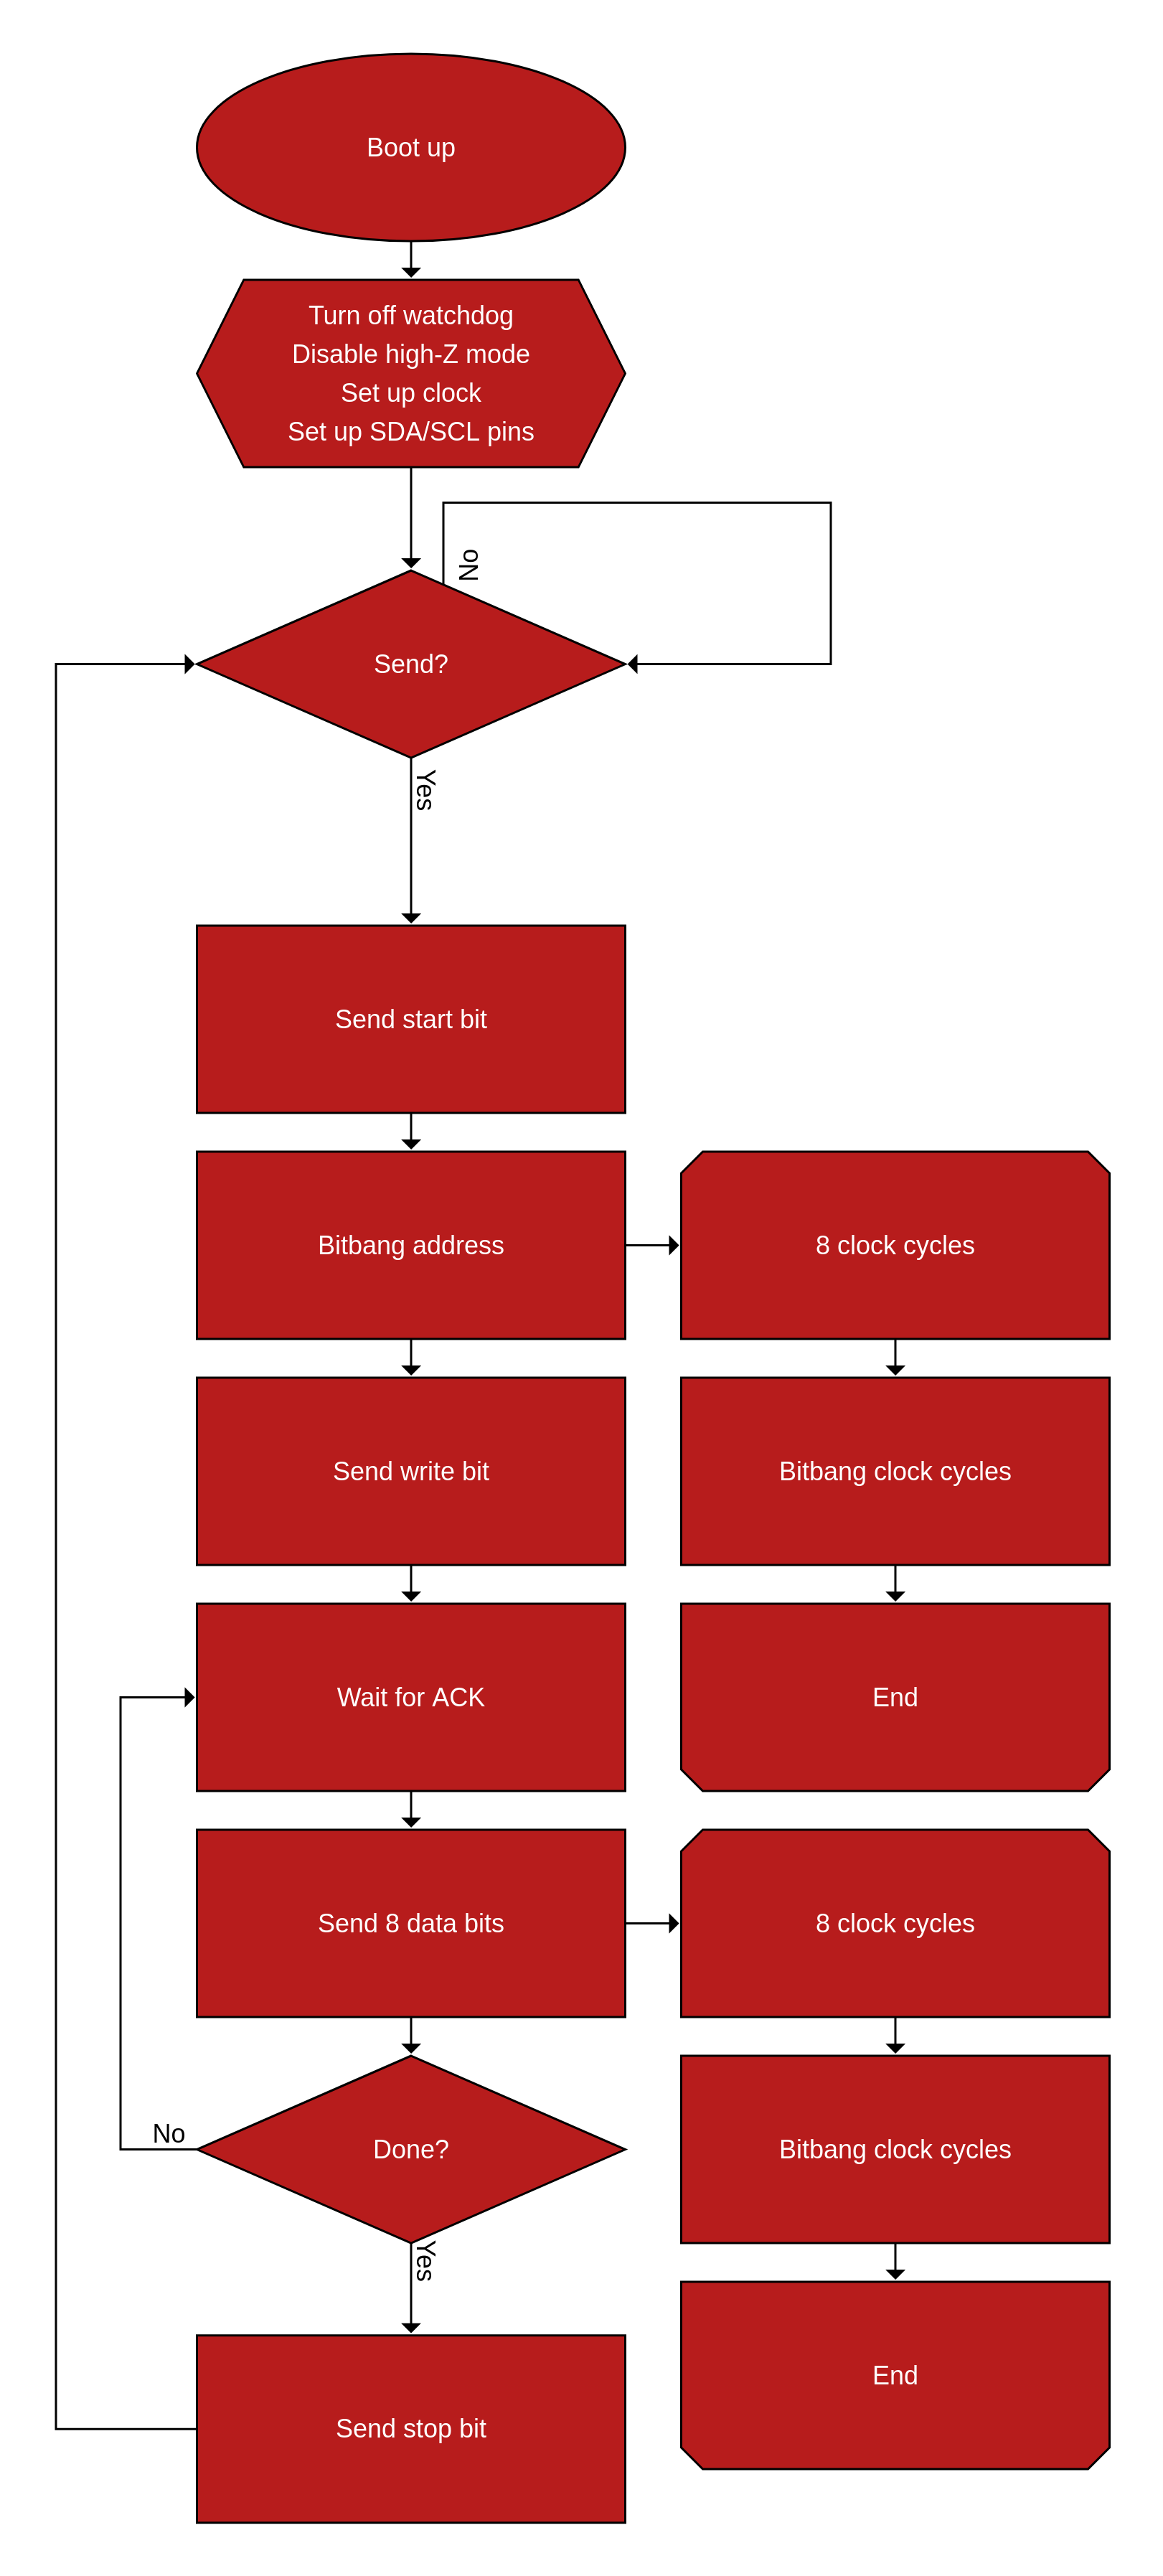
\includegraphics[width = \textwidth]{graph.png}
\captionsetup{format = hang, width = 0.75\textwidth}
\caption{MSP430FR2355 Flowchart}
\label{fig:Flowchart}
\end{figure}
\end{centering}


%************ Bibliography ************
\newpage
\bibliography{Final}
\bibliographystyle{ieeetr}




% \begin{center}
% 	\begin{minipage}{0.6\linewidth} % Adjust the minipage width to accomodate for the length of algorithm lines
% 		\begin{algorithm}[H]
% 			\caption{Lattice Boltzmann Method} % Algorithm name
% 			\label{alg:KeyPress}   % optional label to refer to
% 			\algsetup{indent=4em}
% 			\begin{algorithmic}[H]
% 				\STATE IN: $(LAT, \nu, u_0) \gets$ Lattice Pts, Viscosity, Initial Velocities
%
% 				\hrulefill
% 				\medskip
%
% 				\STATE \# Inverse of time constant, $\tau$:
% 				\STATE $\Omega = \Omega(\nu)$
% 				\STATE \# Weights are known for D2Q9:
% 				\STATE const w $\gets$ weights::Array
% 				\STATE $f_i(x_0, t_0) = f_i($LAT, weights, $\nu, u_0)$
% 				\STATE $\rho \gets$ calc\_densities()
% 				\STATE $u_x, u_y \gets$ calc\_velocities()
% 				\STATE object $\gets$ gen\_object()
% 				\STATE initialize\_plots()
%
% 				\hrulefill
% 				\medskip
%
% 				\STATE \textbf{StartLoop:}
% 				\STATE \# Do one step for each point and handle object collisions
% 				\FOR{($pts \in$ LAT)}
% 					\STATE $f_i(x_i) \gets f_i(x_i + e_i \cdot \delta t)$
% 					\IF{($x_i \in$ object)}
% 						\STATE $f_i(x_i) \gets$ boundary\_condition($f_i$)
% 					\ENDIF
% 				\ENDFOR
% 				\STATE
%
% 				\hrulefill
% 				\medskip
%
% 				\STATE \# Do collisions between fluid elements
% 				\STATE \# then check inlet/outlet BCs:
% 				\STATE $\rho \gets$ calc\_densities()
% 				\STATE $u_x, u_y \gets$ calc\_velocities()
% 				\FOR{$pts \in$ LAT}
% 					\STATE $f_i(x_i) \gets$ update($f_i, \Omega, u_x, u_y$)
% 					\IF{($pt \in$ border)}
% 						\STATE \# Force flow @ initial velocity
% 						\STATE $f_i(x_i) \gets$ force\_flow($f_i$, $u_0$)
% 					\ENDIF
% 				\ENDFOR
% 				\STATE
%
% 				\hrulefill
% 				\medskip
%
% 				\STATE \# Get curl of macro velocity fields to
% 				\STATE \# calculate vorticity
% 				\STATE curl\_vals $\gets$ curl($u_x, u_y$)
% 				\STATE update\_plot(curl\_vals, object)
%
% 				\STATE \textbf{goto: StartLoop}
% 			\end{algorithmic}
% 		\end{algorithm}
% 	\end{minipage}
% \end{center}


%--------------------------------------------------------------------------
%--------------------------------------------------------------------------
%----------------------- END DOCUMENT -------------------------------------
%--------------------------------------------------------------------------
%--------------------------------------------------------------------------
\end{document}
